These notes are from a guest lecture by Gaurav Arya in IAP 2023.

\subsection{Introduction}

In this class, we've learned how to take derivatives of all sorts of crazy functions.
Recall one of our first examples:
\begin{equation}
    f(A) = A^2,
\end{equation}
where $A$ is a matrix.
%complicated: both 
To differentiate this function, we had to go back to the drawing board, and
ask: 
\begin{question}
If we perturb the input slightly, how does the output change?
\label{question:perturb}
\end{question}
To this end, we wrote down something like:
\begin{equation}
    \delta f = (A+\delta A)^2 - A^2 = A (\delta A) + (\delta A) A + \underbrace{(\delta A)^2}_{\text{neglected}}.
\end{equation}
We called $\delta f$ and $\delta A$ \emph{differentials} in the limit where $\delta A$ became arbitrarily small. 
We then had to ask: 
\begin{question}
What terms in the differential can we neglect?
\label{question:neglect}
\end{question}
We decided that $(\delta A)^2$ should be neglected, 
justifying this by the fact
that $(\delta A)^2$ is ``higher-order''. We were left with the derivative operator $\delta A \mapsto 
A(\delta A) + (\delta A) A$: the best possible \emph{linear} approximation
to $f$ in a neighbourhood of $A$. At a high level, the main challenge here was dealing with
complicated input and output spaces: $f$ was matrix-valued, and also matrix-accepting. 
We had to ask ourselves: in this case, what should the notion of a derivative even mean?

In this lecture, we will face a similar challenge, but with an even weirder type of function.
This time, the output of our function will be \emph{random}. Now, we need to 
revisit the same questions. If the output is random,
how can we describe its response to a change in the input?
And how can we form a useful notion of derivative?

\subsection{Stochastic programs}

More precisely, we will consider random, or \emph{stochastic}, functions $X$ with real input
$p \in \mathbb{R}$ and real-valued random-variable output. As a map, we can write $X$ as
\begin{equation}
    p \mapsto X(p),
\end{equation}
where $X(p)$ is a random variable.  (To keep things simple, we'll take $p \in \mathbb{R}$ and $X(p) \in \mathbb{R}$ in this chapter, though of course they could be generalized to other vector spaces as in the other chapters. For now, the randomness is complicated enough to deal with.)

The idea is that we can only \emph{sample} from $X(p)$, according to some distribution of numbers with probabilities that depend upon $p$.   One simple example would be sampling real numbers uniformly (equal probabilities) from the interval $[0,p]$. As a more complicated example, suppose $X(p)$ follows the \emph{exponential distribution} with scale $p$, corresponding to randomly sampled real numbers $x \ge 0$ whose probability decreases proportional to $e^{-x/p}$.  This can be denoted $X(p) \sim \operatorname{Exp}(p)$, and implemented in Julia by:

\begin{minted}{jlcon}
julia> using Distributions

julia> sample_X(p) = rand(Exponential(p))
sample_X (generic function with 1 method)
\end{minted}
We can take a few samples:
\begin{minted}{jlcon}
julia> sample_X(10.0)
1.7849785709142214

julia> sample_X(10.0)
4.435847397169775

julia> sample_X(10.0)
0.6823343897949835

julia> mean(sample_X(10.0) for i = 1:10^9) # mean = p
9.999930348291866
\end{minted}

If our program gives a different output each time, what could a useful notion of derivative be?
Before we try to answer this, let's ask \emph{why} we might want to take a derivative.
%we need to ask if this is even a well-posed problem.
%If a function gives a different output every time, what could a derivative possibly signify? 
%And what useful information could the derivative give us?
The answer is that we may be very interested in \emph{statistical properties} of random functions,
i.e.~values that can be expressed using \emph{averages}.  Even if a function is stochastic, its \emph{average} (``expected value''), assuming the average exists, can be a deterministic function of its parameters that has a conventional derivative.

So, why not take the average \emph{first}, and then take the ordinary derivative of this average?  This simple approach works for very basic stochastic functions (e.g.~the exponential distribution above has expected value $p$, with derivative $1$), but runs into practical difficulties for more complicated distributions (as are commonly implemented by large computer programs working with random numbers).
\begin{remark}
    It is often much easier to produce an ``unbiased estimate'' $X(p)$ of a statistical quantity than to compute it exactly. (Here, an unbiased estimate means that $X(p)$ averages out to our statistical quantity of interest.)
\end{remark}


For example, in deep learning, the ``variational autoencoder'' (VAE) is a very common architecture
that is inherently stochastic. It is easy to get a stochastic \emph{unbiased estimate} of the loss function by running a
random simulation $X(p)$: the loss function $L(p)$ is then the ``average'' value of $X(p)$, denoted by the \emph{expected value} $\EE[X(p)]$.
However, computing the loss $L(p)$ exactly would require integrating over all possible outcomes, which usually is  impractical.
Now, to train the VAE, we also need to differentiate $L(p)$, i.e.~differentiate $\EE[X(p)]$ with respect to $p$!

Perhaps more intuitive examples can be found in the physical sciences, where randomness may be baked into
your model of a physical process.
In this case, it's hard to get around the fact that you need to deal with stochasticity! 
For example, you may have two particles that interact with an \emph{average} rate of $r$.
But in reality, the times when these interactions actually occur follow a stochastic process. 
(In fact, the time until the first interaction might be exponentially distributed, with scale $1/r$.)
And if you want to (e.g.) fit the parameters of your stochastic model to real-world data, it's once again very useful to have derivatives.

If we can't compute our statistical quantity of interest exactly, it seems unreasonable to assume we
can compute its derivative exactly. However, we could hope to stochastically \emph{estimate} its derivative.
That is, if $X(p)$ represents the full program that produces an unbiased estimate of our statistical quantity, 
%our notion of derivative helps describe how our random variable $X(p)$ is changing with respect to
%$p$, 
here's one property we'd definitely like our notion of derivative to have: 
we should be able to construct from it an unbiased gradient estimator\footnote{For more discussion of these concepts, see (e.g.) the review article ``Monte Carlo gradient estimation in machine learning'' (2020) by Mohamed \textit{et al.} (\url{https://arxiv.org/abs/1906.10652}).} $X'(p)$ satisfying
\begin{equation}
    \EE[X'(p)] = \EE[X(p)]' = \frac{\partial \EE[X(p)]}{\partial p}.
\end{equation}
Of course, there are infinitely many such estimators. For example, given any estimator $X'(p)$ we can add any other random variable that has zero average without changing the  expectation value. But in practice there are two additional considerations: (1) we want $X'(p)$ to be easy to compute/sample (about as easy as $X(p)$), and (2) we want the \emph{variance} (the ``spread'') of $X'(p)$ to be small enough that we don't need too many samples to estimate its average accurately (hopefully no worse than estimating $\EE[X(p)]$).

\subsection{Stochastic differentials and the reparameterization trick}

Let's begin by answering our first question (Question \ref{question:perturb}): how does $X(p)$ respond to a change in $p$?
Let us consider a specific $p$ and write down a \emph{stochastic differential}, taking a small but non-infinitesimal $\delta p$ to avoid thinking about infinitesimals for now:
\begin{equation}
    \delta X(p) = X(p + \delta p) - X(p),
\end{equation}
where $\delta p$ represents an arbitrary small change in $p$.
What sort of object is $\delta X(p)$?

Since we're subtracting two random variables, it ought to itself be a random variable.
However, $\delta X(p)$ is still not fully specified! We have only specified 
the marginal distributions of $X(p)$ and $X(p+\delta p)$: to be able to subtract the two,
we need to know their \emph{joint distribution}.

One possibility is to treat $X(p)$ and $X(p + \delta p)$ as independent. 
This means that $\delta X(p)$ would be constructed as the difference of independent samples.
Let's see how samples from $\delta X(p)$ would look like in this case! 
\begin{minted}{jlcon}
julia> sample_X(p) = rand(Exponential(p))
sample_X (generic function with 1 method)

julia> sample_δX(p, δp) = sample_X(p + δp) - sample_X(p)
sample_δX (generic function with 1 method)

julia> p = 10; δp = 1e-5;

julia> sample_δX(p, δp)
-26.000938718875904

julia> sample_δX(p, δp)
-2.6157162001718092

julia> sample_δX(p, δp)
6.352622554495474

julia> sample_δX(p, δp)
-9.53215951927184

julia> sample_δX(p, δp)
1.2232268930932104
\end{minted}
We can observe something a bit worrying: even for a very tiny $\delta p$ (we chose $\delta p = 10^{-5}$),
$\delta X(p)$ is still fairly large: essentially as large as the original random variables.
This is not good news if we want to construct a derivative from $\delta X(p)$: we would rather see its magnitude 
getting smaller and smaller with $\delta p$, like in the non-stochastic case.  Computationally, this will make it very difficult to determine $\EE[X(p)]'$ by averaging \texttt{sample\_δX(p, δp) / δp} over many samples: we'll need a huge number of samples because the \emph{variance}, the ``spread'' of random values, is huge for small~$\delta p$.

Let's try a different approach. It is natural to think of $X(p)$ for all $p$ as forming a \emph{family} of random variables, all 
defined on the same \emph{probability space}.
A probability space, with some simplification, is a sample space $\Omega$, with a probability distribution $\mathbb{P}$ defined 
on the sample space.
From this point of view, each $X(p)$ can be expressed as a function $\Omega \to \mathbb{R}$. 
To sample from a particular $X(p)$, we can imagine drawing a random $\omega$ from $\Omega$ according to $\PP$, and then
plugging this into $X(p)$, i.e.~computing $X(p)(\omega)$.  (Computationally, this is how most distributions are actually implemented: you start with a primitive pseudo-random number generator for a very simple distribution,\footnote{Most computer hardware cannot generate numbers that are actually random, only numbers that \emph{seem} random, called ``pseudo-random'' numbers.  The design of these random-seeming numeric sequences is a subtle subject, steeped in number theory, with a long history of mistakes.  A famous ironic quotation in this field is (Robert Coveyou, 1970): ``Random number generation is too important to be left to chance.''} e.g.~drawing values $\omega$ uniformly from $\Omega = [0,1)$, and then you build other distributions on top of this by transforming $\omega$ somehow.) Intuitively, all of the ``randomness'' resides in the probability space, and crucially 
$\mathbb{P}$ does not depend on $p$: as $p$ varies, $X(p)$ just becomes a different 
\emph{deterministic} map on $\Omega$. 


The crux here is that all the $X(p)$ functions now depend on a shared source of randomness: the random draw of $\omega$.
This means that $X(p)$ and $X(p+\delta p)$ have a nontrivial joint distribution: what does it look like?

For concreteness, let's study our exponential random variable $X(p) \sim \operatorname{Exp}(p)$ from above.  Using the ``inversion sampling'' parameterization,
it is possible to choose $\Omega$ to be $[0,1)$ and $\mathbb{P}$ to be the uniform distribution over
$\Omega$; for any distribution, we can construct $X(p)$ to be a corresponding nondecreasing function over $\Omega$ (given by the inverse of $X(p)$'s cumulative probability distribution). 
Applied to $X(p) \sim \operatorname{Exp}(p)$, the inversion method gives $X(p)(\omega) = -p \log{(1-\omega)}$.  This is implemented below, and is a theoretically equivalent way
of sampling $X(p)$ compared with the opaque \texttt{rand(Exponential(p))} function we used above:
\begin{minted}{julia}
julia> sample_X2(p, ω) = -p * log(1 - ω)
sample_X2 (generic function with 1 method)

julia> # rand() samples a uniform random number in [0,1)
julia> sample_X2(p) = sample_X2(p, rand()) 
sample_X2 (generic function with 2 methods)

julia> sample_X2(10.0)
8.380816941818618

julia> sample_X2(10.0)
2.073939134369733

julia> sample_X2(10.0)
29.94586208847568

julia> sample_X2(10.0)
23.91658360124792
\end{minted}
Okay, so what does our joint distribution look like?
% Both $X(p+\delta p)$ and $X(p)$ are random variables.
% However, before we can subtract them, we need to clear about what probability space we are working on,
% and in particular what the joint distribution of $X(p+\delta p)$ and $X(p)$ is.
% For example, if $X(p) \sim \operatorname{Exp}(p)$, we can write 
% where $U \sim \operatorname{Unif}(0, 1)$ is a uniform distribution from 0 to 1:
% Since $U$ is independent of $p$, we can use the same $U$ for all $p$, giving us a joint distribution
% over the $X(p)$:
% Since $X(p)$ all belong to the same probability space, they all share the same source of randomness.
\begin{figure}[t]
    \centering
    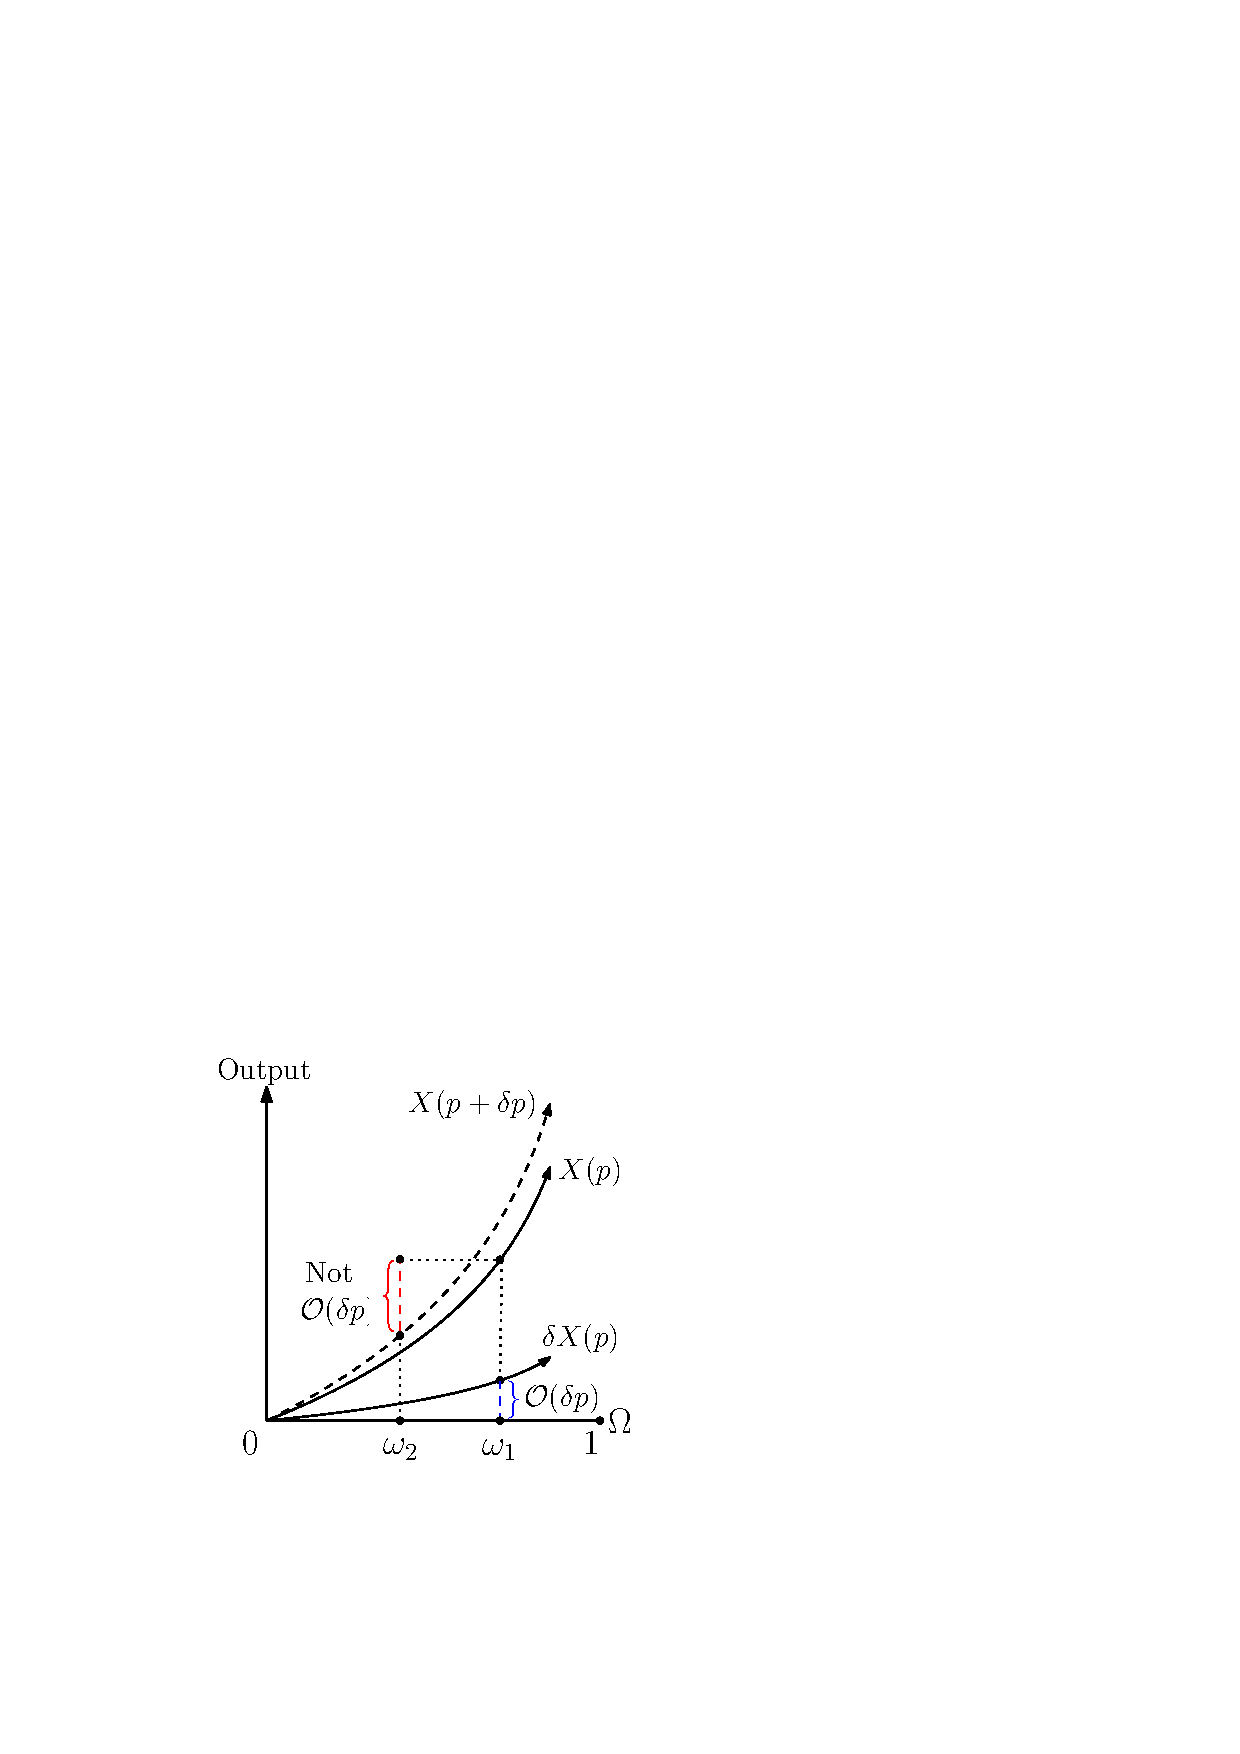
\includegraphics[width=0.4\textwidth]{figures/exp_for_matrixcalc.pdf}
    \caption{For $X(p) \sim \operatorname{Exp}(p)$ parameterized via the inversion method, we can write $X(p)$, $X(p+\delta p)$, and
    $\delta X(p)$ as functions from $\Omega = [0,1] \to \mathbb{R}$, defined on a probability space with
    $\mathbb{P} = \operatorname{Unif}(0,1)$.}
    \label{fig:exp}
\end{figure}
As shown in Figure~\ref{fig:exp}, we can plot $X(p)$ and $X(p+\delta p)$ as functions over $\Omega$.
To sample the two of them jointly, we use the \emph{same} choice of $\omega$:
thus, $\delta X(p)$ can be formed by subtracting the two functions \emph{pointwise} at each $\Omega$. 
Ultimately, $\delta X(p)$ is itself a random variable over the same probability space, sampled in the same way: 
we pick a random $\omega$ according to $\mathbb{P}$, and evaluate $\delta X(p)(\omega)$, using the function $\delta X(p)$ depicted above.
Our first approach with independent samples is depicted in red in Figure~\ref{fig:exp}, while our second approach is in blue.
We can now see the flaw of the independent-samples approach: the $\mathcal{O}(1)$-sized ``noise'' from the independent samples washes out
the $\mathcal{O}(\delta p)$-sized ``signal''.
% So we now have a joint distribution over the $X(p)$, and thus $\delta X(p)$ is well-defined: it is just
% another random variable over the sample probability space. 
% We sample from $\delta X(p)$ in the same way: 

What about our second question (Question \ref{question:neglect}): how can actually take the limit of $\delta p \to 0$ and compute the derivative?
The idea is to differentiate $\delta X(p)$ at each fixed sample $\omega \in \Omega$. 
In probability theory terms, we take the limit of random variables $\delta X(p) / \delta p$
as $\delta p \to 0$:
\begin{equation}
    X'(p) = \lim_{\delta p \to 0} \frac{\delta X(p)}{\delta p}.
\end{equation}
For $X(p) \sim \operatorname{Exp}(p)$ parameterized via the inversion method, we get:
\begin{equation}
    X'(p)(\omega) = \lim_{\delta p \to 0} \frac{-\delta p\log{(1-\omega)}}{\delta p} = -\log{(1-\omega)}.
\end{equation}
Once again, $X'(p)$ is a random variable over the same probability space.
The claim is that $X'(p)$ is the notion of derivative we were looking for! Indeed, $X'(p)$ is itself in fact
a valid gradient estimator:
\begin{equation}
    \EE[X'(p)] = \EE\left[ \lim_{\delta p \to 0} \frac{\delta X(p)}{\delta p}\right] \stackrel{?}{=} 
\lim_{\delta p \to 0} \frac{\EE[\delta X(p)]}{\delta p} = 
    \frac{\partial \EE[X(p)]}{\partial p}.
    \label{eq:exchange} 
 \end{equation} 
Rigorously, one needs to justify the interchange of limit and expectation in the above.
In this chapter, however, we will be content with a crude empirical justification:
\begin{minted}{julia}
julia> X′(p, ω) = -log(1 - ω)
X′ (generic function with 1 method)

julia> X′(p) = X′(p, rand())
X′ (generic function with 2 methods)

julia> mean(X′(10.0) for i in 1:10000)
1.011689946421105
\end{minted}
So $X'(p)$ does indeed average to 1, which makes sense since the expectation of $\operatorname{Exp}(p)$ is $p$, which has derivative 1 for any choice of $p$. However, 
% (However, the number 1 also averages to 1, so this is hardly a rigorous proof!)
the crux is that this notion of derivative 
also works for more complicated random variables that can be formed via \emph{composition} of simple ones such as an exponential random variable. In fact, it turns out to obey the same chain rule as usual!

% does not lose any information about how the full random variable $X(p)$ reacts to changes in $p$. 
% This means it can be composed to form derivative estimators of more complicated functions. In fact, it turns out to obey the same chain rule as usual! 
% In contrast, if our notion of derivative was simply $\frac{\delta \EE[X(p)]}{\delta p} = 1$, we would not be able
% to have a chain rule that enables differentiation of more complicated functions.

Let's demonstrate this. Using the dual numbers introduced in Chapter~\ref{sec:AD}, we can differentiate the expectation of the square of a sample 
from an exponential distribution \emph{without} having an analytic expression for this quantity.
(The expression for $X'$ we derived is already implemented as a dual-number rule in Julia by the \texttt{ForwardDiff.jl} package.)
The primal and dual values of the outputted dual number are samples from the joint distribution of $(X(p), X'(p))$.
\begin{minted}{julia}
julia> using Distributions, ForwardDiff: Dual

julia> sample_X(p) = rand(Exponential(p))^2
sample_X (generic function with 1 method)

julia> sample_X(Dual(10.0, 1.0)) # sample a single dual number!
Dual{Nothing}(153.74964559529033,30.749929119058066)

julia> # obtain the derivative!
julia> mean(sample_X(Dual(10.0, 1.0)).partials[1] for i in 1:10000)
40.016569793650525
\end{minted}
Using the ``reparameterization trick'' to form a gradient estimator, as we have done here, is a fairly old idea. It is also called 
the ``pathwise'' gradient estimator. Recently,
it has become very popular in machine learning due to its use in VAEs [e.g.~Kingma~\& Welling (2013): \url{https://arxiv.org/abs/1312.6114}], and lots of resources
can be found online on it. Since composition simply works by the usual chain rule, it also works in reverse mode, and
can differentiate functions far more complicated than the one above!
%Our treatment here is arguably much less concise than it could be, but emphasizes some key conceptual points and sets the
% stage for understanding what goes wrong with discreteness, which is what we turn to next.
% Emphasize composability, this is called the reparameterization trick, also enables reverse-mode AD.
% Relating back to $X(p)$ and $X(p+\delta p)$, the intuition is that we have used the same underlying randomness to sample 
% both the original program and perturbed programs.

% \begin{equation}
%     X(p) = \operatorname{Exp}(1).
% \end{equation}
\subsection{Handling discrete randomness}

So far we have only considered a continuous random variable. Let's see how the picture changes for a discrete random 
variable! Let's take a simple Bernoulli variable $X(p) \sim \operatorname{Ber}(p)$, which is 1 with probability $p$ and
0 with probability $1-p$.
\begin{minted}{jlcon}
julia> sample_X(p) = rand(Bernoulli(p))
sample_X (generic function with 1 method)

julia> p = 0.5
0.6

julia> sample_X(δp) # produces false/true, equivalent to 0/1
true


julia> sample_X(δp)
false

julia> sample_X(δp)
true
\end{minted}
The parameterization of a Bernoulli variable is shown in Figure 2.
Using the inversion method once again, the parameterization of a Bernoulli variable looks like a step function:
for $\omega < 1-p$, $X(p)(\omega) = 0$, while for $\omega \geq 1-p$, $X(p)(\omega) = 1$.

Now, what happens when we perturb $p$? Let's imagine perturbing $p$ by a positive amount $\delta p$.
As shown in Figure 2, something qualitatively very different has happened here. At nearly every $\omega$ except a small region
of probability $\delta p$, the output does not change. Thus, the quantity $X'(p)$ we defined in the previous subsection 
(which, strictly speaking, was defined by an "almost-sure" limit that neglects regions of probability 0)
is 0 at every $\omega$: after all, for every $\omega$, there exists small enough $\delta p$ such that $\delta X(p)(\omega) = 0$.

\begin{figure}[t]
    \centering
    \begin{subfigure}[b]{0.4\textwidth}
        \centering 
        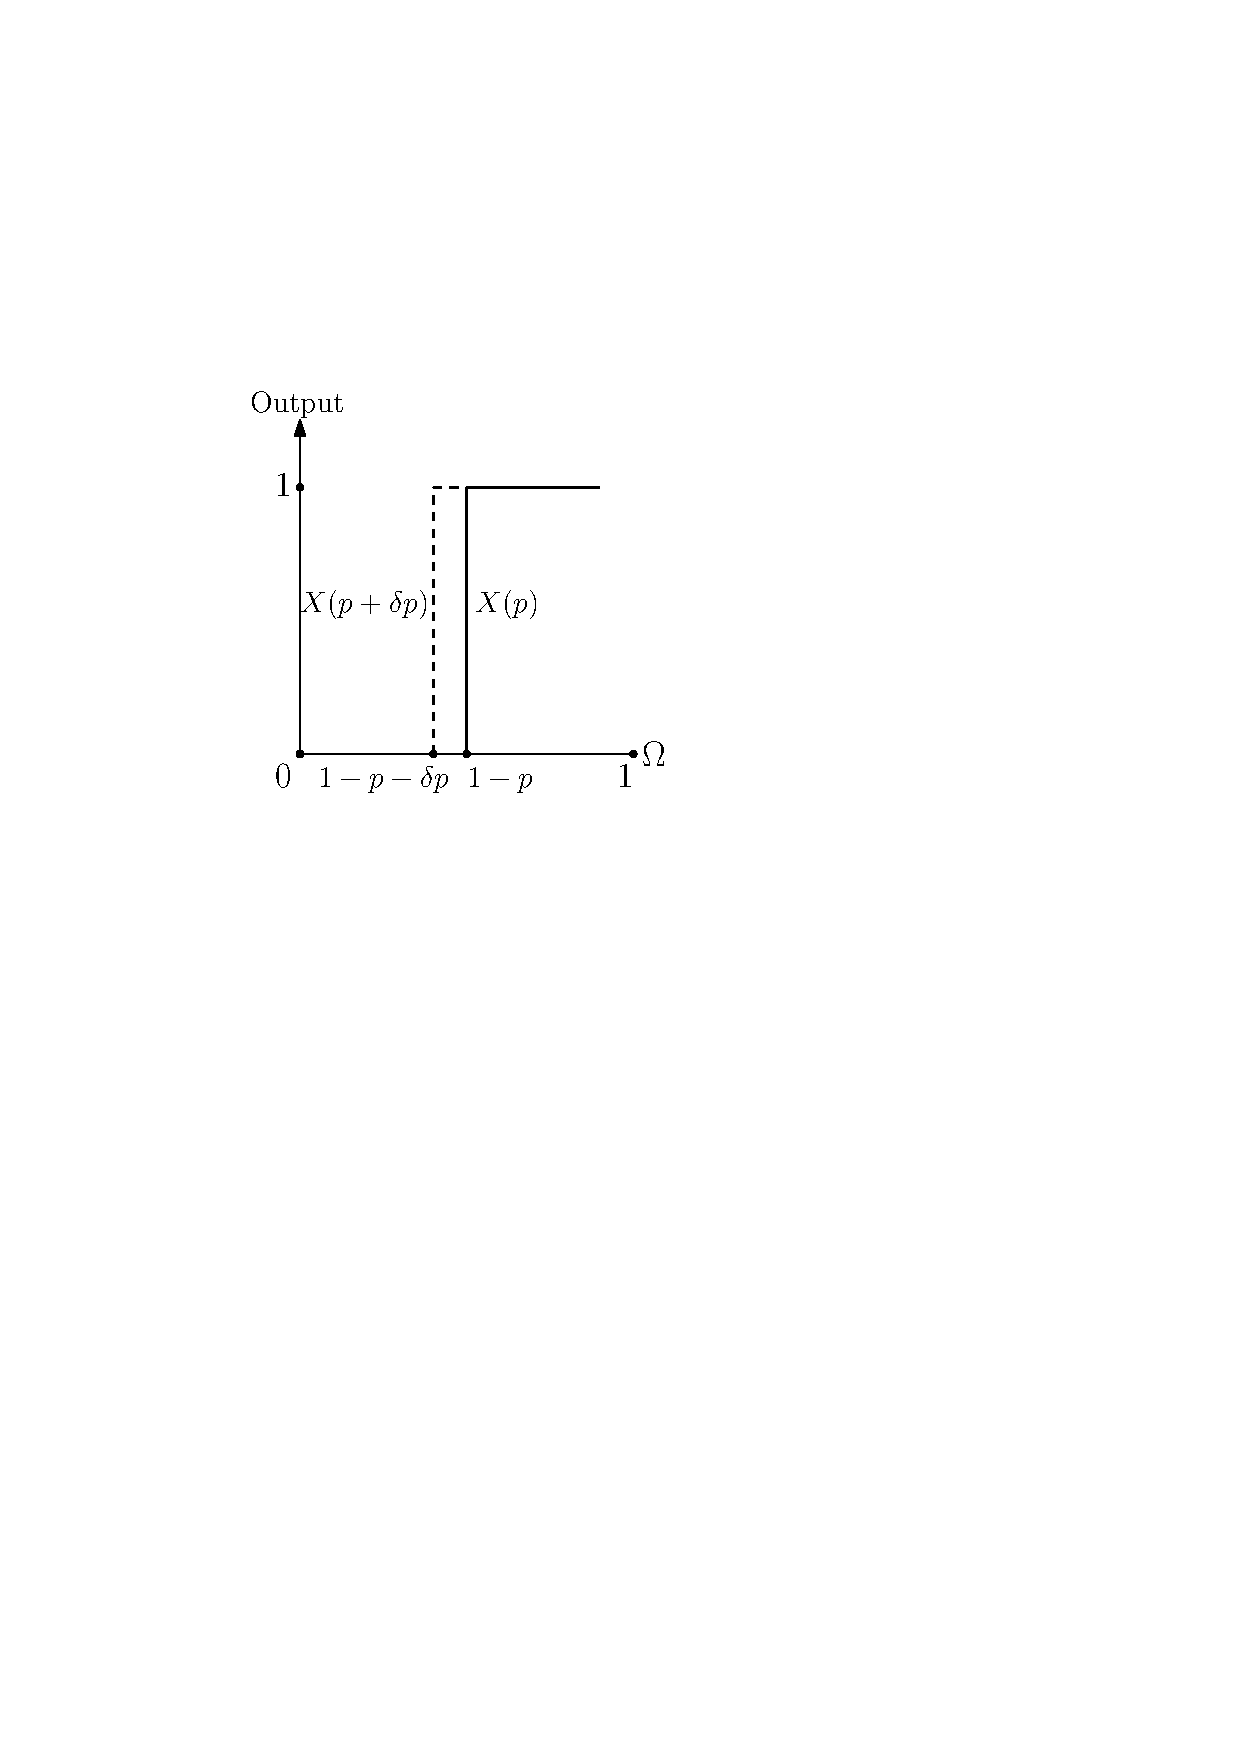
\includegraphics[height=4.5cm]{figures/ber1_for_matrixcalc.pdf}
        \label{fig:ber1} 
    \end{subfigure} 
    \begin{subfigure}[b]{0.4\textwidth}
        \centering
        
\includegraphics[height=4.5cm]{figures/ber2_for_matrixcalc.pdf}
        \label{fig:ber2}
    \end{subfigure}
    \caption{For $X(p) \sim \operatorname{Ber}(p)$ parameterized via the inversion method, 
    plots of $X(p)$, $X(p+\delta p)$, and $\delta X(p)$ as functions $\Omega: [0, 1] \to \mathbb{R}$. }
\end{figure}


However, there is certainly an important derivative contribution to consider here. 
The expectation of a Bernoulli is $p$, so we would expect the derivative to be 1: but $\EE[X'(p)] = \EE[0] = 0$. What has gone wrong is that, although $\delta X(p)$ is 0 with tiny probability, the value of $\delta X(p)$
on this region of tiny probability is 1, which is \emph{large}. In particular, it does not approach 0 as $\delta p$
approaches 0. Thus, to develop a notion of derivative of $X(p)$, we need to somehow capture these large jumps with ``infinitesimal''
probability. 

A recent (2022) publication (\url{https://arxiv.org/abs/2210.08572}) by the author of this chapter (Gaurav Arya), together with Frank~Sch\"afer, Moritz~Schauer, and Chris~Rackauckas, worked to extend the above ideas to develop a notion of 
``stochastic derivative'' for discrete randomness, implemented by a software package called \texttt{StochasticAD.jl} that performs automatic differentiation of such stochastic processes. 
It generalizes the idea of dual numbers to stochastic \emph{triples}, which include a third component to capture exactly these large jumps. For example, the stochastic triple of a Bernoulli variable might look like:
\begin{minted}{jlcon}
julia> using StochasticAD, Distributions
julia> f(p) = rand(Bernoulli(p)) # 1 with probability p, 0 otherwise
julia> stochastic_triple(f, 0.5) # Feeds 0.5 + δp into f
StochasticTriple of Int64:
0 + 0ε + (1 with probability 2.0ε)
\end{minted}
Here, $\delta p$ is denoted by $\upepsilon$,  imagined to be an ``infinitesimal unit'', so that the above triple indicates a flip from 0 to 1 with probability that has derivative $2$. 

However, many aspects of these problems are still difficult, and there are a lot of improvements awaiting future developments! If you're
interested in reading more, you may be interested in the paper and our package linked above, as well as the 2020 review article by Mohamed \textit{et~al.} (\url{https://arxiv.org/abs/1906.10652}), which is a great survey
of the field of gradient estimation in general.

At the end of class, we considered a differentiable random walk example with \texttt{StochasticAD.jl}. Here it is!
% A key idea is as follows: recall that the derivative can be thought of as the 
% best ``linear'' approximation to a function. But in the case of a Bernoulli, it is the \emph{place where the step occurs}
% that appears to be moving approximately (in this case, exactly) linearly in $\delta p$. Thus, this is what we want
% to differentiate: more precisely, we want to differentiate the probability that a jump occurs. In~\cite{arya2022automatic},
% we generalize the idea of dual numbers to stochastic \emph{triples} which allow 

% In~\cite{arya2022automatic},
% we try to develop this idea to fruition by considering the derivative 
% we develop 
% Why could we have expected this?

% The remaining challenge becomes to  This is certainly a difficult problem, that remains far from solved. 
%Now write down differential... some notational differentials, we will simply use $\delta p$ to denote
%a change in $p$, rather than $\delta p$.

% Recall (2), had to strip out linear, here what is linear?

% Just like before, composable:

\begin{minted}{jlcon}
julia> using Distributions, StochasticAD

julia> function X(p)
           n = 0
           for i in 1:100
               n += rand(Bernoulli(p * (1 - (n+i)/200)))
           end
           return n
       end
X (generic function with 1 method)

julia> mean(X(0.5) for _ in 1:10000) # calculate E[X(p)] at p = 0.5
32.6956

julia> st = stochastic_triple(X, 0.5) # sample a single stochastic triple at p = 0.5
StochasticTriple of Int64:
32 + 0δp + (1 with probability 74.17635818221052δp)

julia> derivative_contribution(st) # derivative estimate produced by this triple
74.17635818221052

julia> # compute d/dp of E[X(p)] by taking many samples
julia> mean(derivative_contribution(stochastic_triple(f, 0.5)) for i in 1:10000)
56.65142976168479
\end{minted}

